\documentclass{../includes/TechDoc}
\usepackage[T1]{fontenc}
\usepackage[utf8]{inputenc}
\usepackage[pdftex]{graphicx}
\DeclareGraphicsRule{*}{mps}{*}{}

\title{Мобильное приложение для сообщений о бытовых проблемах студентов в общежитии}
\author{Студент группы БПИ-194}{В. А. Анненков}
\academicTeacher{Доцент департамента программной инженерии факультета компьютерных наук}{Х. М. Салех}

\documentTitle{Программа и методика испытаний}
\documentCode{RU.17701729.04.03-01 51 01-1}

\begin{document}
    \maketitle

    \begin{abstract}
        Программа и методика испытаний – это документ, назначение которого — подтверждение выполнения требований некоторого программного продукта.

        Настоящая Программа и методика испытаний предназначена для правильной организации работы Android-приложения «Мобильное приложение для сообщений о бытовых проблемах студентов в общежитии».

        Данная Программа и методика испытаний содержит следующие разделы: «Объект испытаний», «Цель испытаний», «Требования к программе», «Требования к программной документации», «Средства и порядок испытаний», «Методы испытаний». В зависимости от особенностей документа допускается вводить дополнительные разделы.

        В разделе «Объект испытаний» указывают наименование, область применения и обозначение испытуемой программы.

        В разделе «Цель испытаний» должна быть указана цель проведения испытаний.

        В разделе «Требования к программе» должны быть указаны требования, подлежащие проверке во время испытаний и заданные в техническом задании на программу.

        В разделе «Требования к программной документации» должны быть указаны состав программной документации, предъявляемой на испытания, а также специальные требования, если они заданы в техническом задании на программу.

        В разделе «Средства и порядок испытаний» должны быть указаны технические и программные средства, используемые во время испытаний, а также порядок проведения испытаний.

        В разделе «Методы испытаний» должны быть приведены описания используемых методов испытаний.

    \end{abstract}

    \newpage

    \tableofcontents


    \section{Объект испытаний}

    \subsection{Наименование испытуемой программы}

    \subsubsection{Наименование программы на русском языке}

    Мобильное приложение для сообщений о бытовых проблемах студентов в общежитии.

    \subsubsection{Наименование программы на английском языке}

    Mobile Application for Informing about Household Problems in Dormitory.

    \subsection{Область применения испытуемой программы}

    Программа может быть использована высшим учебным заведением для обеспечения централизованной связи со студентами, а
    также для информирования студентов о последних новостях в своих общежитиях.


    \section{Цель испытаний}

    Цель проведения испытаний — проверка функциональных характеристик программы на соответствие надёжности и стабильности
    мобильного приложения, а так же серверной составляющей, изложенным в документе <<Техническое задание>>.


    \section{Требования к программе}

    Разрабатываемое приложение должно:

    \begin{enumerate}
        \item выполнять авторизацию и регистрацию в сервисе;
        \item выполнять отправлять защитный код на почту в доменах @hse.ru или @edu.hse.ru;
        \item выдавать ошибку, при попытке авторизоваться с почтой в другом домене;
        \item отображать экран с введением информации о профиле при первичной авторизации;
        \item отображать главную страницу со следующими данными:
        \begin{enumerate}
            \item общие данные пользователя;
            \item важные уведомления;
            \item новости;
            \item предстоящие события;
            \item популярные вопросы;
        \end{enumerate}
        \item давать пользователю возможность редактировать свой профиль;
        \item отображать список персональных обращений;
        \item давать пользователю возможность создавать/дополнять/удалять обращения;
        \item давать пользователю возможность общаться с агентами тех. поддержки в режиме чата;
        \item отображать общий чат общежития;
        \item давать пользователю возможность отправить сообщение в общий чат общежития;
        \item давать пользователю возможность обновить общий чат общежития.
    \end{enumerate}


    \section{Требования к программной документации}

    \subsection{Состав программной документации, предъявляемой на испытания}

    В состав программной документации должны входить следующие компоненты:
    \begin{enumerate}
        \item Техническое задание (ГОСТ 19.201-78)
        \item Программа и методика испытаний (ГОСТ 19.301-78)
        \item Пояснительная записка (ГОСТ 19.404-79)
        \item Руководство оператора (ГОСТ 19.505-79)
        \item Текст программы (ГОСТ 19.401-78)
    \end{enumerate}

    \subsection{Специальные требования}

    Документы к программе должны быть выполнены в соответствии с ГОСТ 19.106-78 и ГОСТами к каждому виду документа (см. п. 5.1.);

    Пояснительная записка должна быть загружена в систему Антиплагиат через LMS «НИУ ВШЭ». Лист, подтверждающий загрузку пояснительной записки, сдается в учебный офис вместе со всеми материалами не позже, чем за день до защиты курсовой работы.;

    Вся документация также воспроизводится в печатном виде, она должна быть подписана академическим руководителем образовательной программы 09.03.04 «Программная инженерия», руководителем разработки и исполнителем перед сдачей курсовой работы в учебный офис не позже одного дня до защиты;

    Документация и программа также сдается в электронном виде в формате .pdf или .docx. в архиве формата .zip или .rar;

    За один день до защиты комиссии все материалы курсового проекта:
    \begin{itemize}
        \item техническая документация,
        \item программный проект,
        \item исполняемый файл,
        \item отзыв руководителя
    \end{itemize}
    должны быть загружены одним или несколькими архивами в проект дисциплины «Курсовой проект 2017-2018» в личном кабинете в информационной образовательной среде LMS (Learning Management System) НИУ ВШЭ.


    \section{Средства и порядок испытаний}

    \subsection{Технические средства, используемые во время испытаний}

    Во время проведения испытаний были использованы следующие технические средства:
    \begin{enumerate}
        \item мобильный телефон с сенсорным экраном;
        \item стабильное интернет подключение;
        \item более 11 МБ оперативной памяти.
    \end{enumerate}

    \subsection{Программные средства, используемые во время испытаний}

    Во время проведения испытаний были использованы следующие программные средства:
    \begin{enumerate}
        \item операционная система iOS 11 и выше.
    \end{enumerate}

    \subsection{Порядок проведения испытаний}

    Порядок проведения испытаний должен включать:
    \begin{enumerate}
        \item проверку требований к функциональным характеристикам;
        \item проверку требований к интерфейсу;
        \item проверку требований к формату входных и выходных данных;
        \item проверку требований к надёжности;
        \item проверку требований к программной документации.
    \end{enumerate}


    \section{Методы испытаний}

    \subsection{Испытание выполнения требований к функциональным характеристикам}

    Для проведения испытаний требуется запустить программу на эмуляторе или физическом устройстве под управлением операционной системы iOS\@.

    \begin{enumerate}
        \item При вводе почты в домене @hse.ru или @edu.hse.ru код подтверждения успешно отправляется на введённую почту (Рис.~\ref{fig:login_code_success}).
        \begin{figure}[ht]
            \centering
            \frame{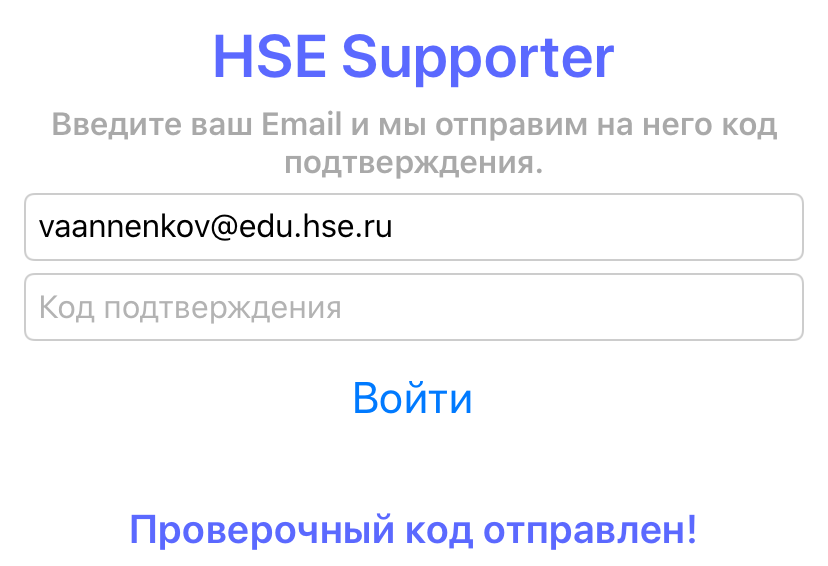
\includegraphics[width=0.63\linewidth]{images/login_code_success.png}}
            \caption{Успешная отправка кода подтверждения}
            \label{fig:login_code_success}
        \end{figure}

        \item При первом входе отображается страница с вводом необходимых данных для работы приложения (Рис.~\ref{fig:wait_page})
        \begin{figure}[ht]
            \centering
            \frame{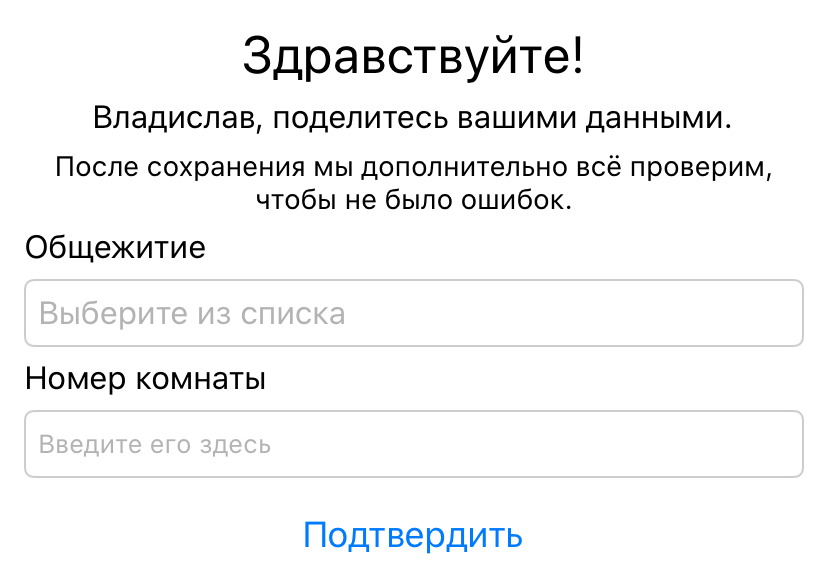
\includegraphics[width=0.63\linewidth]{images/wait_page.png}}
            \caption{Страница для ввода данных пользователя}
            \label{fig:wait_page}
        \end{figure}

        \item После успешной авторизации отображается главная страница со всей необходимой информацией (Рис.~\ref{fig:main_page})
        \begin{enumerate}
            \item общие данные пользователя;
            \item важные уведомления;
            \item новости;
            \item предстоящие события;
            \item популярные вопросы;
        \end{enumerate}
        \begin{figure}[ht]
            \centering
            \frame{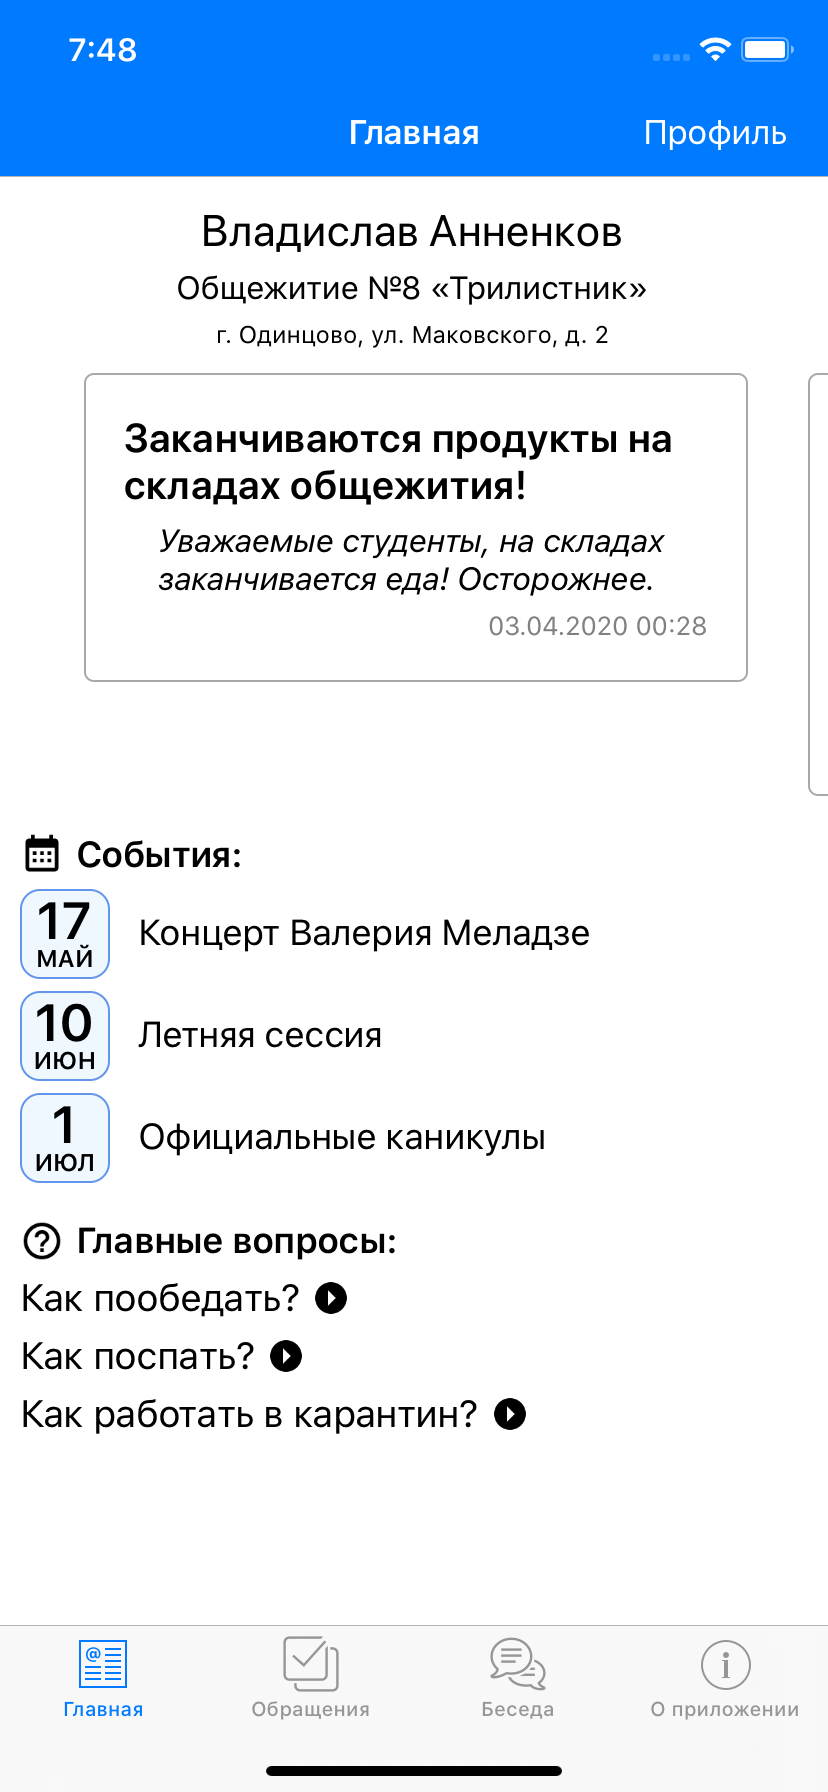
\includegraphics[width=0.3\linewidth]{images/main_page.png}}
            \caption{Главная страница со всеми требуемыми разделами}
            \label{fig:main_page}
        \end{figure}

        \item Если возникает ошибка при загрузке главной страницы, сообщение сообщает об этом (Рис.).

        \item При нажатии на кнопку <<Профиль>> отображается экран с полями для редактирования (Рис.).
        Поля <<Имя>> и <<Фамилия>> являются некликабельными, поля <<Общежитие>> и <<Комната>> можно поменять.

        \item При нажатии на пункт меню <<Обращения>> отображается список обращений.
        Сначала этот список пустой (Рис.).

        \item Обращение можно создать, нажав на кнопку <<Создать>> и заполнив форму (Рис.).

        \item После успешного создания обращения оно отображается в списке (Рис.).

        \item Если при создании возникает ошибка, приложение сообщает об этом (Рис.).

        \item Чтобы открыть подробную информацию об обращении, на него требуется нажать.
        На странице обращения (Рис.) можно отправить сообщение, заполнив форму и нажав на кнопку отправки.
        Для обновления обращения можно потянуть страницу вверх до появления индикатора загрузки (Рис.).

        \item Обращение можно удалить, если потянуть его влево и нажать на кнопку <<Удалить>> (Рис.).

        \item При нажатии на пункт меню <<Беседа>> отображается общий чат общежития (Рис.).

        \item На странице беседы можно отправить сообщение, заполнив форму и нажав на кнопку отправки.

        \item На странице беседы можно обновить список сообщений, нажав на кнопку обновления.

        \item Если при отправке сообщения или обновлении беседы возникает ошибка, приложение сообщает об этом (Рис.).
    \end{enumerate}

    \subsection{Испытание выполнения требований к интерфейсу}

    Для проведения испытаний требуется запустить программу на эмуляторе или физическом устройстве под управлением операционной системы iOS\@.

    \subsection{Испытание выполнения требований к формату входных и выходных данных}

    Для проведения испытаний требуется запустить программу на эмуляторе или физическом устройстве под управлением операционной системы iOS\@.

    \begin{enumerate}
        \item На экране авторизации: при вводе неверных данных (Рис.~\ref{ris:login_error_text}) или при вводе Email не в домене @hse.ru или @edu.hse.ru (Рис.~\ref{ris:login_error_email}) приложение отображает ошибку.
        \begin{figure}[ht]
            \begin{center}
                \begin{minipage}[ht]{0.49\linewidth}
                    \frame{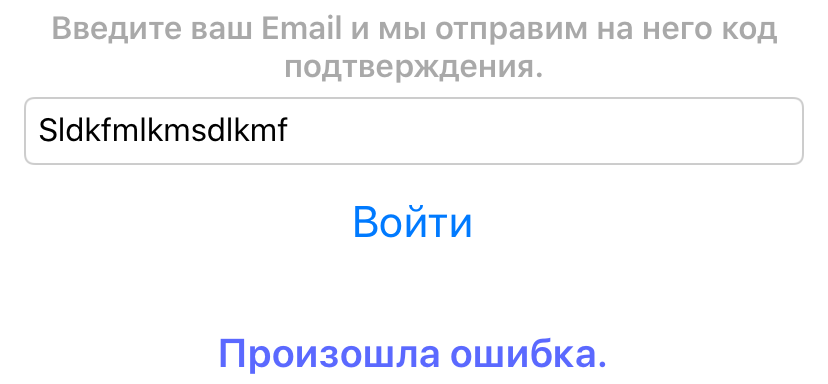
\includegraphics[width=1\linewidth]{images/login_error_text.png}}
                    \caption{Ввод неверных данных} %% подпись к рисунку
                    \label{ris:login_error_text} %% метка рисунка для ссылки на него
                \end{minipage}
                \hfill
                \begin{minipage}[ht]{0.49\linewidth}
                    \frame{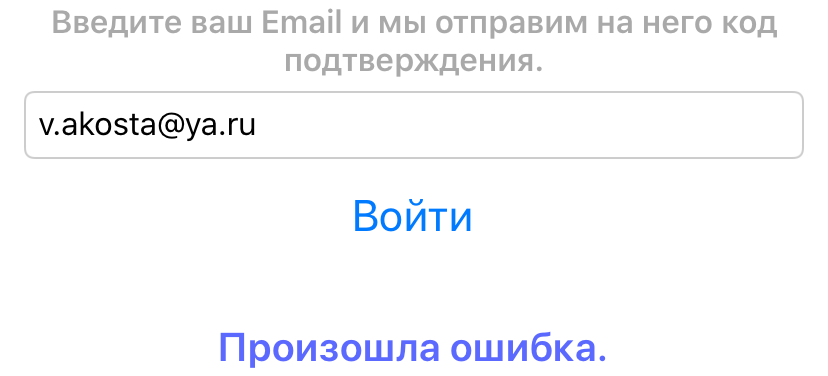
\includegraphics[width=1\linewidth]{images/login_error_email.png}}
                    \caption{Ввод Email не в домене @hse.ru или @edu.hse.ru}
                    \label{ris:login_error_email}
                \end{minipage}
            \end{center}
        \end{figure}

        \item На экране заполнения данных профиля: при отсутствующих значениях приложение просит заполнить все поля (Рис.~\ref{fig:wait_page_empty_labels}).
        \begin{figure}[ht]
            \centering
            \frame{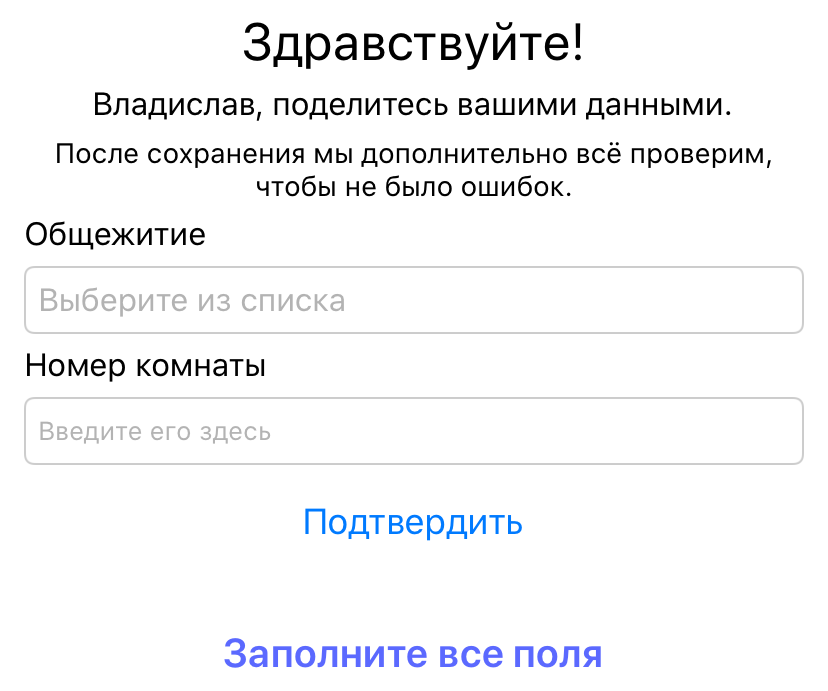
\includegraphics[width=0.7\linewidth]{images/wait_page_empty_labels.png}}
            \caption{Попытка сохранить данные с пустыми полями}
            \label{fig:wait_page_empty_labels}
        \end{figure}

        \item При попытке отправить пустое сообщение в общем чате или в обращении кнопка отправки будет неактивна (Рис.~\ref{fig:input_text}).
        \begin{figure}[ht]
            \centering
            \frame{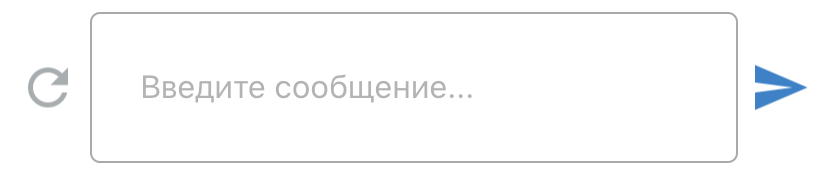
\includegraphics[width=0.8\linewidth]{images/input_text.png}}
            \caption{Поле ввода сообщений в общем чате и в обращении}
            \label{fig:input_text}
        \end{figure}
    \end{enumerate}

    \subsection{Испытание выполнения требований к надёжности}

    Для проведения испытаний требуется воспользоваться программой Postman для имитации HTTP-запросов.
    Требуется убедиться в надёжности REST методов сервера по адресу \url{https://hse-supporter.herokuapp.com/}.

    \begin{enumerate}
        \item При попытке сделать неавторизованный запрос к любым методам, например, /main\_page (Рис.~\ref{ris:api_main_page}), /profile (Рис.~\ref{ris:api_profile}) сервер просит авторизоваться и не отображает информацию.
        \begin{figure}[ht]
            \begin{center}
                \begin{minipage}[ht]{0.49\linewidth}
                    \frame{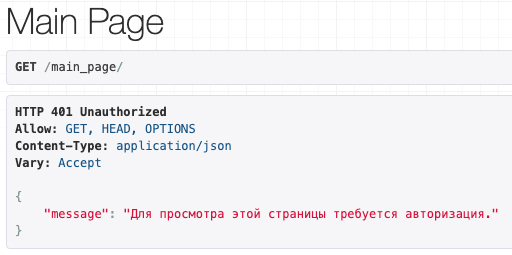
\includegraphics[width=1\linewidth]{images/api_main_page.png}}
                    \caption{Ответ на неавторизованный запрос к методу /main\_page} %% подпись к рисунку
                    \label{ris:api_main_page} %% метка рисунка для ссылки на него
                \end{minipage}
                \hfill
                \begin{minipage}[ht]{0.49\linewidth}
                    \frame{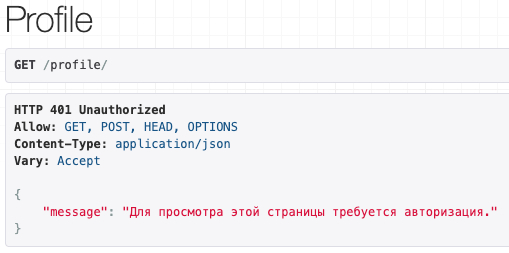
\includegraphics[width=1\linewidth]{images/api_profile.png}}
                    \caption{Ответ на неавторизованный запрос к методу /profile}
                    \label{ris:api_profile}
                \end{minipage}
            \end{center}
        \end{figure}

        \item При запросе на получение списка общежитий, авторизованный пользователь может просматривать
        сообщения из общего чата только своего общежития (Рис.~\ref{ris:api_dormitory_messages}).
        \begin{figure}[ht]
            \centering
            \frame{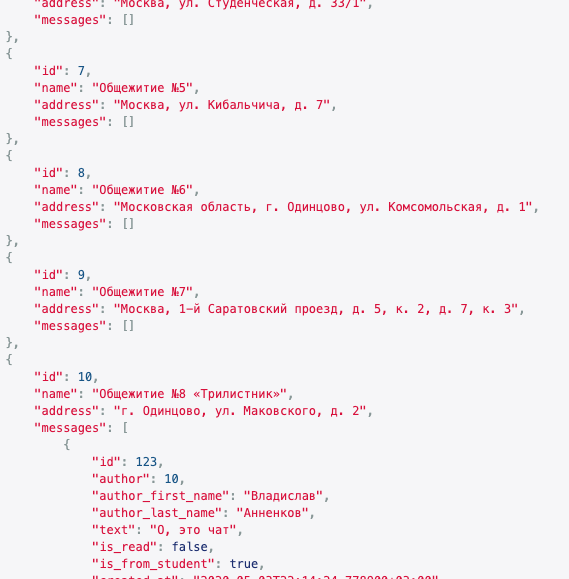
\includegraphics[width=0.49\linewidth]{images/api_dormitory_messages.png}}
            \caption{Список общежитий, где сообщения отображаются только у общежития №8, в котором проживает авторизованный пользователь}
            \label{ris:api_dormitory_messages}
        \end{figure}

        \item При запросе на просмотр списка обращений (Рис.~\ref{ris:api_problem_list}) сервер возвращает только обращения пользователя.
        В базе данных в это время находятся и другие обращения (Рис.~\ref{ris:api_full_problem_list}) от сторонних пользователей, которые сервер не отображает.
        \begin{figure}[ht]
            \centering
            \frame{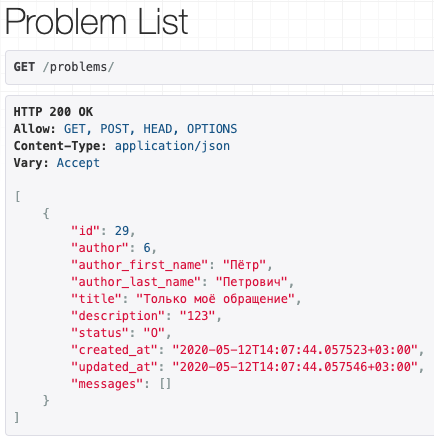
\includegraphics[width=0.9\linewidth]{images/api_problem_list.png}}
            \caption{Список обращений, которые возвращает сервер}
            \label{ris:api_problem_list}
        \end{figure}
        \begin{figure}[ht]
            \centering
            \frame{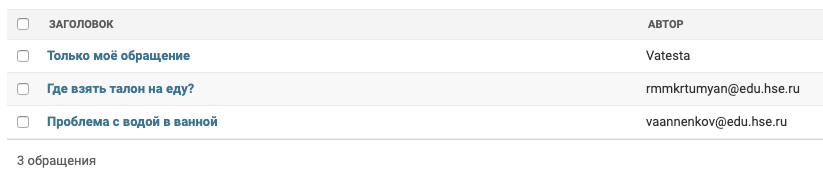
\includegraphics[width=1\linewidth]{images/api_full_problem_list.png}}
            \caption{Полный список обращений в базе данных}
            \label{ris:api_full_problem_list}
        \end{figure}
    \end{enumerate}

    \subsection{Испытание выполнения требований к программной документации}

    Полный пакет документации проверяется вручную на наличие подписей студента, научного и академического руководителей, а также на соответствие ГОСТу.



    \begin{thebibliography}{3}
        \bibitem{gost}Единая система программной документации – М.: ИПК, Издательство стандартов, 2000, 125 стр.
        \bibitem{lms} LMS [Электронный ресурс] URL: \url{https://lms.hse.ru/} (Дата обращения: 30.04.2020, режим доступа: свободный)
        \bibitem{ruz} РУЗ [Электронный ресурс] URL: \url{https://ruz.hse.ru/} (Дата обращения: 30.04.2020, режим доступа: свободный)
        \bibitem{github} GitHub [Электронный ресурс] URL: \url{https://github.com/} (Дата обращения: 30.04.2020, режим доступа: свободный)
        \bibitem{microsoft} Документация Microsoft [Электронный справочник] URL: \url{https://docs.microsoft.com/ru-ru/} (Дата обращения: 30.04.2020, режим доступа: свободный)
        \bibitem{stackoverflow} StackOverflow [Электронный ресурс] URL: \url{https://stackoverflow.com/} (Дата обращения: 30.04.2020, режим доступа: свободный)
    \end{thebibliography}

    \registrationList

\end{document}
